\documentclass[aspectratio=169]{beamer}
% Shared preamble for ml/ slide decks.
% Each lecture .tex starts with:
%   \documentclass[aspectratio=169]{beamer}
%   \input{../preamble}
% Compile from inside the chapter folder so \input{../preamble} resolves.

\usetheme{default}
\usecolortheme{dove}

\setbeamertemplate{navigation symbols}{}
\setbeamertemplate{footline}{%
  \hfill{\large\insertframenumber\,/\,\inserttotalframenumber}\hspace{0.8em}\vspace{0.5em}%
}

% Project palette (existing, kept for backwards compatibility with deferred/*)
\definecolor{popblue}{RGB}{52, 101, 164}
\definecolor{sampred}{RGB}{204, 0, 0}
\definecolor{paramgreen}{RGB}{0, 140, 70}
\definecolor{warnred}{RGB}{180, 40, 40}
\definecolor{orange1}{RGB}{220, 120, 0}
\definecolor{violet1}{RGB}{120, 50, 160}
\definecolor{lightbg}{RGB}{245, 245, 250}

% Armenian flag palette (use these for any 3-color highlight; per CLAUDE.md).
% "Nice versions": slightly de-saturated from the official spec for slide use,
% so they don't burn out under projector colors. Originals kept as *_pure.
\definecolor{armred}{RGB}{200, 30, 40}      % nice red (official #D90012 muted)
\definecolor{armblue}{RGB}{30, 70, 160}     % nice blue (official #0033A0 muted)
\definecolor{armorange}{RGB}{230, 160, 30}  % nice orange (official #F2A800 muted)
\definecolor{armred_pure}{HTML}{D90012}     % official Armenian flag red
\definecolor{armblue_pure}{HTML}{0033A0}    % official Armenian flag blue
\definecolor{armorange_pure}{HTML}{F2A800}  % official Armenian flag orange

\setbeamercolor{frametitle}{fg=popblue}
\setbeamercolor{title}{fg=popblue}

\usepackage{pgfplots}
\usepackage{tikz}
\usetikzlibrary{shapes, arrows.meta, positioning, calc, decorations.pathreplacing, patterns, matrix}
\pgfplotsset{compat=1.18}
\usepackage{amsmath, amssymb, amsfonts}
\usepackage{bm}
\usepackage{dsfont}
\usepackage{array}
\usepackage{pifont}
\usepackage{colortbl}
\usepackage{fontenc}

% Callout boxes. Purely additive - existing decks are unaffected.
% Usage: \begin{tcolorbox}[colback=armblue!8, colframe=armblue, boxrule=0.6pt, arc=2pt,
%                          title=\textbf{Key idea}] ... \end{tcolorbox}
% Palette convention (ml/SLIDE_STYLE.md): armblue=key idea, armred=trap/warning,
% paramgreen=takeaway or "Next", armorange=watch-out.
\usepackage[most]{tcolorbox}

% Cleaner table rules (\toprule, \midrule, \bottomrule). Also purely additive.
\usepackage{booktabs}

% \cancel{...} for struck-through terms in derivations (added 2026-08-11 for the
% importance-sampling frame in ch11_rl, where the dynamics cancel). Purely additive.
\usepackage{cancel}

% Minimal ML notation macros (subset of slds-lmu latex-math/basic-ml.tex).
% Kept here so we don't have to inline-expand every \thetav, \xv, etc.
% when porting upstream slides.
\newcommand{\R}{\mathds{R}}
\newcommand{\N}{\mathds{N}}
\newcommand{\E}{\mathds{E}}
\newcommand{\Xspace}{\mathcal{X}}
\newcommand{\Yspace}{\mathcal{Y}}
\newcommand{\Hspace}{\mathcal{H}}
\newcommand{\D}{\mathcal{D}}
\newcommand{\Dtrain}{\mathcal{D}_{\text{train}}}
\newcommand{\Dtest}{\mathcal{D}_{\text{test}}}
\newcommand{\xv}{\mathbf{x}}
\newcommand{\yv}{\mathbf{y}}
\newcommand{\Xmat}{\mathbf{X}}
\newcommand{\id}{\mathbf{I}}
\newcommand{\thetav}{\bm{\theta}}
\newcommand{\thetah}{\hat{\bm{\theta}}}
\newcommand{\lamv}{\bm{\lambda}}
\newcommand{\fx}{f(\xv)}
\newcommand{\fxt}{f(\xv \,|\, \bm{\theta})}
\newcommand{\fxi}{f\!\left(\xv^{(i)}\right)}
\newcommand{\fh}{\hat{f}}
\newcommand{\fxh}{\hat{f}(\xv)}
\newcommand{\yh}{\hat{y}}
\newcommand{\yih}{\hat{y}^{(i)}}
% \xi clashes with the Greek letter \xi; write \xv^{(i)} inline instead.
\newcommand{\yi}[1][i]{y^{(#1)}}
\newcommand{\xyi}[1][i]{\left(\xv^{(#1)},\, y^{(#1)}\right)}
\newcommand{\thx}{\bm{\theta}^\top \xv}
\newcommand{\sumin}{\sum_{i=1}^{n}}
\newcommand{\sumjp}{\sum_{j=1}^{p}}
\newcommand{\Lxy}{L\!\left(y, \fx\right)}
\newcommand{\Lxyi}{L\!\left(\yi, \fxi\right)}
\newcommand{\risk}{\mathcal{R}}
\newcommand{\riske}{\mathcal{R}_{\text{emp}}}
\newcommand{\risket}{\mathcal{R}_{\text{emp}}(\bm{\theta})}
\newcommand{\riskt}{\mathcal{R}(\bm{\theta})}
\newcommand{\riskr}{\mathcal{R}_{\text{reg}}}
\newcommand{\argmin}{\mathop{\mathrm{arg\,min}}}
\newcommand{\argmax}{\mathop{\mathrm{arg\,max}}}
\newcommand{\eps}{\varepsilon}


\graphicspath{{fig/}{../00_shared/fig/}{../00_shared/fig/borrowed/welchlabs/}}

% callout boxes, matching the chapter's fcolorbox house pattern (LLM-1 to LLM-7)
\newcommand{\keybox}[1]{\fcolorbox{armblue}{armblue!8}{\parbox{0.97\linewidth}{\small #1}}}
\newcommand{\trapbox}[1]{\fcolorbox{armred}{armred!8}{\parbox{0.97\linewidth}{\small #1}}}
\newcommand{\takebox}[1]{\fcolorbox{paramgreen}{paramgreen!8}{\parbox{0.97\linewidth}{\small #1}}}
\newcommand{\watchbox}[1]{\fcolorbox{armorange}{armorange!12}{\parbox{0.97\linewidth}{\small #1}}}

\newcommand{\sectiontransition}[2]{%
  \begin{frame}[plain]
    \vfill
    \begin{center}
      {\Huge\bfseries\color{popblue} #1}\\[1.1em]
      {\large #2}
    \end{center}
    \vfill
  \end{frame}}

\newcommand{\src}[1]{{\scriptsize\color{gray} #1}}

\title{Scaling Laws and Emergence}
\subtitle{How big, how much data, and what appears}
\author{}
\date{}

\begin{document}

\begin{frame}[plain]
  \titlepage
  \begin{center}\scriptsize\color{gray}
    LLM chapter, session 8. Toy numbers unless a slide says otherwise.
  \end{center}
\end{frame}

% ============================================================ WHERE WE ARE (py_src/llm_roadmap.py)
\begin{frame}{Where we are: one forward pass}
  \begin{center}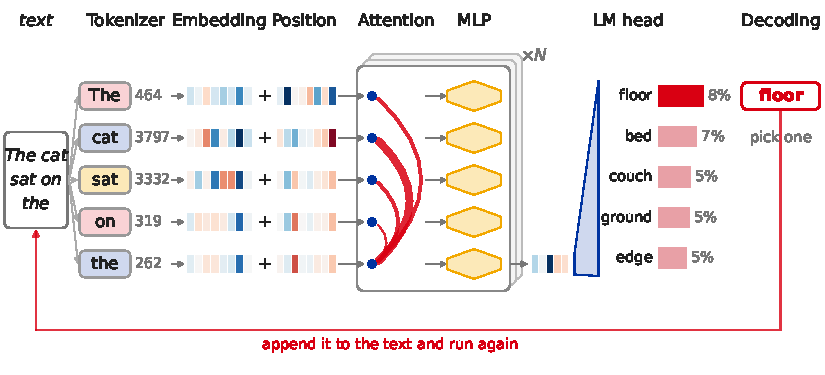
\includegraphics[width=\linewidth]{roadmap_scaling_pass.pdf}\end{center}
  \vskip -2pt
  {\small The pass is built and LLM-7 trained it. Today: how big to make it, and on how much text.}
\end{frame}

\begin{frame}{Where we are: the life of a model}
  \begin{center}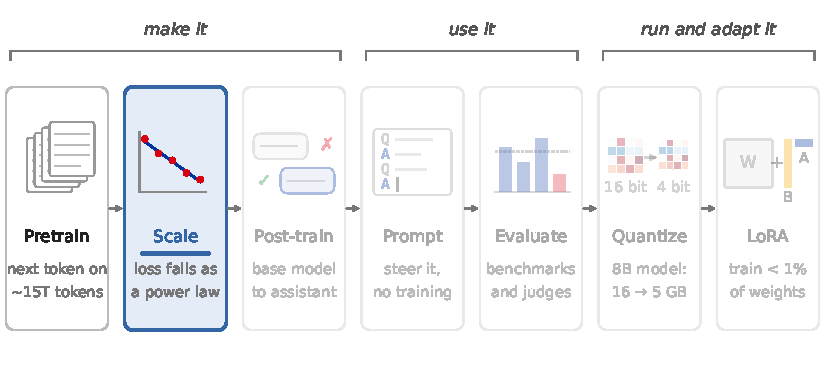
\includegraphics[width=\linewidth]{roadmap_scaling_life.pdf}\end{center}
  \vskip -2pt
  {\small Today: the second box. Pretraining at different sizes, and what changes as you scale.}
\end{frame}

% ============================================================ COLD OPEN
\begin{frame}{Same budget, two models}
  \vskip 4pt
  DeepMind trained two models with about the same amount of compute:

  \vskip 10pt
  \begin{columns}[T]
    \column{0.48\textwidth}
      \keybox{\textbf{Gopher} (2021)\\[3pt] 280 billion parameters\\ trained on 300 billion tokens}
    \column{0.48\textwidth}
      \keybox{\textbf{Chinchilla} (2022)\\[3pt] 70 billion parameters (4$\times$ smaller)\\ trained on
      1.4 trillion tokens (4.7$\times$ more)}
  \end{columns}

  \vskip 14pt
  \trapbox{\textbf{Predict first:} on a broad knowledge test (MMLU: multiple-choice questions in 57
  subjects, four options each, so guessing gets 25\%), which one scores higher?}
\end{frame}

\begin{frame}{The small one}
  \vskip 4pt
  \begin{center}
  \begin{tabular}{lccc}
    \toprule
    & \textbf{parameters} & \textbf{tokens} & \textbf{MMLU, \% correct} \\
    \midrule
    Gopher & 280B & 300B & 60.0\% \\
    Chinchilla & 70B & 1.4T & \textbf{67.5\%} \\
    \bottomrule
  \end{tabular}
  \end{center}

  \vskip 8pt
  {\small Compute check with today's rule $C \approx 6ND$ (in a few frames), in FLOPs (floating-point
  operations): $6 \times 280\text{B} \times 300\text{B} = 5.0 \times 10^{23}$ against
  $6 \times 70\text{B} \times 1.4\text{T} = 5.9 \times 10^{23}$. Within 20\% of each other.}

  \vskip 8pt
  \keybox{Gopher was too big for its data. With a fixed budget, a smaller model trained on more
  tokens wins. Today: how to find the right split, and what happens as the budget grows.}
  \vskip 1pt
  \src{Hoffmann et al. (2022), ``Training Compute-Optimal Large Language Models''.}
\end{frame}

\begin{frame}{Outline}
  \tableofcontents
\end{frame}

% ============================================================ 1. POWER LAWS
\section{Loss is a power law}
\sectiontransition{Loss is a power law}{Small steps, but predictable ones.}

\begin{frame}{Bigger is better, predictably}
  \begin{columns}[c]
    \column{0.62\textwidth}
      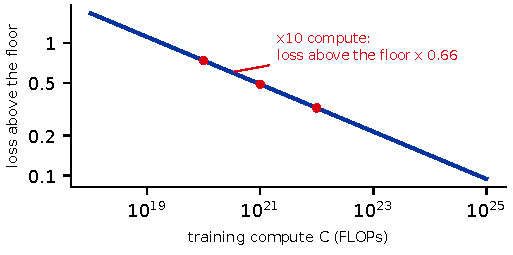
\includegraphics[width=\linewidth]{scal_powerlaw.pdf}
    \column{0.36\textwidth}
      {\small Loss never reaches 0: text has its own randomness, a floor ($E = 1.82$ in the fitted
      law of section 2). Plot what is \emph{above} the floor, at the best model size for each
      budget.

      \vskip 6pt
      A straight line: every $10\times$ of compute multiplies it by the same 0.66.}
  \end{columns}

  \vskip 6pt
  {\small That is a \textbf{power law}. Kaplan et al. (2020) found the same shape for model size
  alone, with data never the limit: exponent 0.076, so doubling $N$ multiplies the loss by
  $2^{-0.076} = 0.949$, about 5\% less. Different quantity, same shape: a fixed factor per
  doubling, or per $10\times$.}

  \vskip 4pt
  \keybox{Each step is small, but the line is so straight that a lab can fit it on small runs and
  predict a run 1,000$\times$ bigger before paying for it.}
\end{frame}

\begin{frame}{The bill: $C \approx 6ND$}
  \vskip 6pt
  Training compute, in floating-point operations:
  \begin{center}
    $C \approx 6 \cdot N \cdot D$ \qquad ($N$ parameters, $D$ training tokens)
  \end{center}
  \begin{itemize}
    \item Forward pass: about 2 FLOPs per parameter per token (one multiply, one add).
    \item Backward pass: about twice that, 4 more (LLM-4's backprop through every layer).
  \end{itemize}

  \vskip 6pt
  \textbf{By hand:} Karpathy's GPT-2 run in LLM-7, 124M parameters on 33B tokens:
  \begin{center}
    $6 \times 124 \times 10^{6} \times 33 \times 10^{9} \approx 2.5 \times 10^{19}$ FLOPs
  \end{center}

  \vskip 4pt
  \keybox{One budget, two knobs. For the same $C$ you can have a bigger model on less text or a
  smaller one on more. Gopher and Chinchilla are two such choices.}
\end{frame}

\begin{frame}{The other bill: memory}
  \begin{center}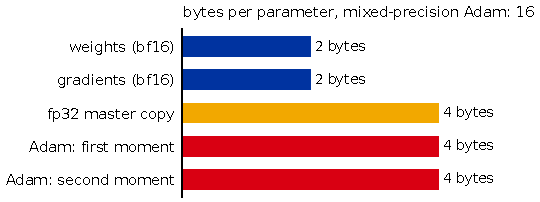
\includegraphics[width=0.66\linewidth]{scal_memory.pdf}\end{center}
  \vskip -4pt
  \small
  \begin{itemize}
    \item Training keeps far more than the weights: their gradients, an exact 32-bit copy for the
      updates, and Adam's two running averages (ch11).
    \item \textbf{By hand:} GPT-2 small, $124\text{M} \times 16$ bytes $\approx$ \textbf{2.0 GB}.
      An 8B model, $8\text{B} \times 16 = $ \textbf{128 GB}: at least two 80 GB GPUs just for this.
      The activations (LLM-4's intermediate values, kept for backprop) come on top. (bf16 is a
      16-bit number format.)
  \end{itemize}
  \vskip 4pt
  \takebox{This number comes back in LLM-13: fine-tuning tricks exist mostly to avoid paying it.}
\end{frame}

% ============================================================ 2. HOW BIG, HOW MUCH DATA
\section{How big, how much data}
\sectiontransition{How big, how much data}{One budget, many ways to spend it.}

\begin{frame}{One budget, many models}
  \begin{columns}[c]
    \column{0.64\textwidth}
      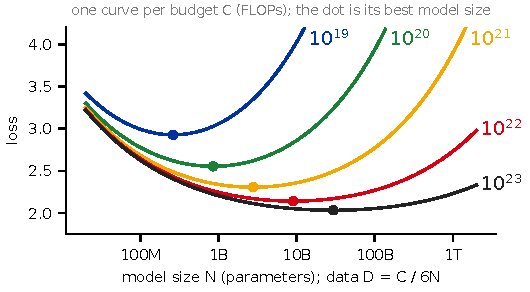
\includegraphics[width=\linewidth]{scal_isoflop.pdf}
    \column{0.34\textwidth}
      {\small Each curve is one budget $C$. Moving right makes the model bigger, so it sees fewer
      tokens ($D = C / 6N$).

      \vskip 6pt
      Too small: not enough capacity. Too big: not enough data. The dot is the best split.}
  \end{columns}

  \vskip 5pt
  \keybox{Chinchilla's rule from these valleys: grow parameters and tokens \textbf{together},
  about \textbf{20 tokens per parameter}. ``For every doubling of model size the number of
  training tokens should also be doubled'' (Hoffmann et al.).}
  {\scriptsize The curves: $L = E + A/N^{\alpha} + B/D^{\beta}$ - the floor, a penalty for a small
  model, a penalty for little data - with the five constants fitted to hundreds of training runs
  (Besiroglu et al.'s 2024 refit).}
\end{frame}

\begin{frame}{By hand: $10^{21}$ FLOPs}
  \vskip 6pt
  Two rules, two unknowns:
  \begin{center}
    $C = 6ND$ \qquad and \qquad $D = 20N$
  \end{center}
  Substitute:
  \begin{center}
    $C = 6 \cdot N \cdot 20N = 120\,N^2 \quad\Longrightarrow\quad
    N = \sqrt{C / 120} = \sqrt{10^{21} / 120} \approx \mathbf{2.9}$ \textbf{billion}
  \end{center}
  \begin{center}
    $D = 20N \approx \mathbf{58}$ \textbf{billion tokens}
  \end{center}

  {\small Check on Chinchilla itself: $C = 5.9 \times 10^{23}$ gives
  $N = \sqrt{5.9 \times 10^{23} / 120} \approx 70$B and $D \approx 1.4$T - the model from the cold
  open.}

  \vskip 4pt
  \keybox{Ten times the compute buys $\sqrt{10} \approx 3.2\times$ the parameters \emph{and}
  $3.2\times$ the tokens - not a 10$\times$ bigger model.}
\end{frame}

\begin{frame}{How to read a claim: the fit}
  \begin{columns}[c]
    \column{0.62\textwidth}
      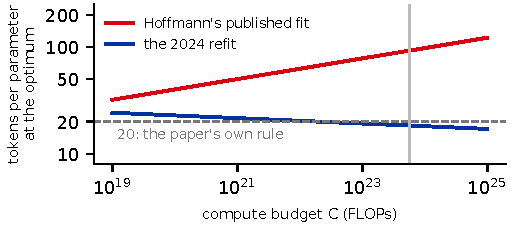
\includegraphics[width=\linewidth]{scal_fit_check.pdf}
    \column{0.36\textwidth}
      {\small Where the minimum of each fitted law sits, as tokens per parameter. The grey line
      marks Chinchilla's budget.}
  \end{columns}

  \vskip 6pt
  {\small The paper's own published constants for $L(N, D)$ put the best split at \textbf{50}
  tokens per parameter at $10^{21}$ FLOPs, and \textbf{93} at Chinchilla's budget - yet Chinchilla
  itself was trained at 20. A 2024 replication refitted the same data: 22 and 18 at those two
  budgets, in line with the paper's other two methods. The headline survived; the published fit
  did not.}

  \vskip 2pt
  \watchbox{Check a fitted law against the claim it is quoted for. Here that meant finding the
  minimum of each curve on the previous slides for both sets of constants: seconds of compute.}
  \src{Besiroglu et al. (2024), ``Chinchilla Scaling: A replication attempt'', arXiv 2404.10102.}
\end{frame}

\begin{frame}{Over-training, on purpose}
  \begin{columns}[c]
    \column{0.62\textwidth}
      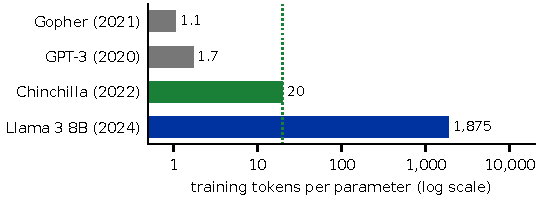
\includegraphics[width=\linewidth]{scal_tokens_per_param.pdf}
    \column{0.36\textwidth}
      {\small Published sizes: Gopher 280B on 300B tokens, GPT-3 175B on 300B, Chinchilla 70B on
      1.4T. Llama 3 8B: over 15T tokens / 8B $\approx$ 1,875 per parameter, 94$\times$ the rule.}
  \end{columns}

  \vskip 8pt
  \begin{itemize}
    \item Chinchilla's rule minimises \textbf{training} compute. But training is paid once;
      every answer costs about $2N$ FLOPs per token (the forward share of $6ND$), for every
      user, for years.
    \item So labs train small models far past 20 tokens per parameter: a slightly higher loss than
      the best split for that training compute, but much cheaper to run.
  \end{itemize}
\end{frame}

% ============================================================ 3. EMERGENCE
\section{Emergence}
\sectiontransition{Emergence}{Abilities that seem to switch on.}

\begin{frame}{Emergent abilities}
  \vskip 6pt
  \begin{itemize}
    \item Wei et al. (2022): an ability is \textbf{emergent} if it is absent in smaller models and
      present in larger ones. Plotted against scale, many tasks look like a switch: chance level
      (no better than guessing), chance level, then suddenly far above it.
    \item A related trend in GPT-3 (2020): the gap between zero-shot and few-shot (LLM-7) widens
      with model size; a few examples in the prompt help large models much more than small ones.
  \end{itemize}

  \vskip 10pt
  \keybox{If abilities appear suddenly, the smooth loss curves of section 1 cannot predict them. That
  would make scaling less predictable than it looked. So: is it really sudden?}
\end{frame}

\begin{frame}{Predict: smooth or sudden?}
  \vskip 8pt
  A toy model family. As the model grows, its \textbf{per-token accuracy} $p$ (the chance each
  answer token is right) rises \emph{smoothly}.

  \vskip 8pt
  The task: a 5-token answer, scored by \textbf{exact match} - all 5 right or nothing.

  \vskip 14pt
  \trapbox{\textbf{Predict first:} what does the exact-match curve look like as the model grows?
  Smooth like $p$, or something else?}
\end{frame}

\begin{frame}{The mirage, by hand}
  \begin{center}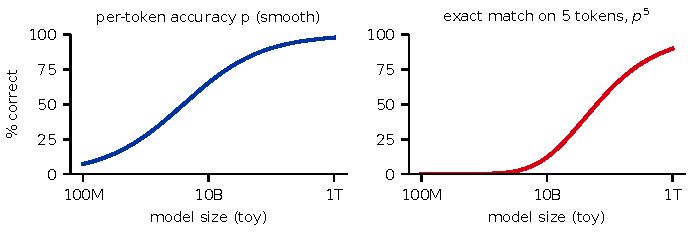
\includegraphics[width=0.84\linewidth]{scal_mirage.pdf}\end{center}
  \vskip -4pt
  {\small Assume each token is right independently, with the same $p$. Exact match needs all five:
  $p^5$. \quad $0.5^5 = 3\%$, \quad $0.7^5 = 17\%$, \quad $0.9^5 = 59\%$, \quad $0.95^5 = 77\%$.
  Almost nothing, then a ``jump'', from a model that improved smoothly all along.}

  \vskip 6pt
  \keybox{Schaeffer et al. (2023): re-score the same models with a continuous metric (per-token
  accuracy, edit distance) and many of the published jumps become smooth curves. Those jumps were
  made by the metric.}
\end{frame}

\begin{frame}{Where the debate stands}
  \vskip 6pt
  \begin{itemize}
    \item The metric explains \textbf{many} jumps, not necessarily all of them; the debate is
      not settled.
    \item For a user the jump is real anyway: an answer with one wrong digit is a wrong answer.
      ``Smooth underneath'' does not help if you need all five tokens.
    \item What it buys you: with the right metric, a capability can be forecast from smaller
      models before it ``appears''.
  \end{itemize}

  \vskip 10pt
  \takebox{When you read ``ability X emerges at size Y'', ask which metric drew the jump.}
\end{frame}

\begin{frame}{Another kind of sudden: grokking}
  \begin{columns}[c]
    \column{0.56\textwidth}
      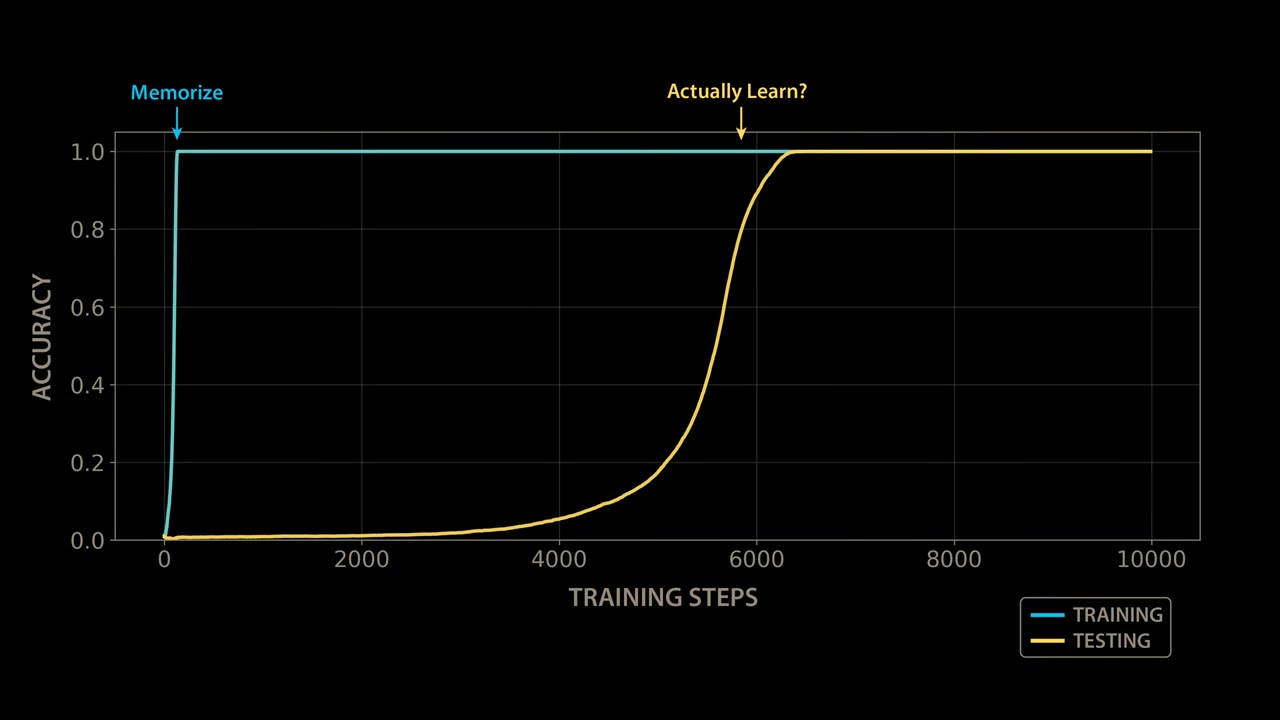
\includegraphics[width=\linewidth]{grokking_curves.jpg}\\
      \src{Welch Labs, ``Grokking'' (2025)}
    \column{0.42\textwidth}
      {\small Welch Labs' own run: a small transformer learning modular addition from part of all
      the pairs. Training accuracy hits 100\% within about 100 steps: it memorised. Test accuracy
      stays near 0 until about 3,000, then reaches 100\% around 6,000 - some 60$\times$ later.

      \vskip 4pt
      In Power et al.'s (2022) original setup (division mod 97, half the pairs) the gap was about
      1,000$\times$.}
  \end{columns}

  \vskip 8pt
  \watchbox{Sudden in \textbf{training time}, not in model size. And the training loss cannot tell
  memorising from generalising: it was already near 0 long before the test accuracy moved.}
\end{frame}

\begin{frame}{A second axis: thinking longer (a preview)}
  \vskip 8pt
  \begin{itemize}
    \item Everything so far spends compute \textbf{before} the model is used: training.
    \item Reasoning models spend it \textbf{while answering}: they write a long chain of thought
      first, and accuracy improves as they are allowed more of it.
    \item That is a second scaling axis - test-time compute. How to prompt for it is LLM-10; how
      such models are trained is the reinforcement-learning chapter.
  \end{itemize}

  \vskip 10pt
  \keybox{Two dials: make the model bigger and train it on more text, or let it think for more
  tokens. They trade off, and both cost compute.}
\end{frame}

% ============================================================ CLOSE
\begin{frame}{Recap}
  \small
  \begin{itemize}
    \item \textbf{Loss is a power law} in size, data and compute: small, predictable steps toward
      a floor.
    \item \textbf{The bills}: $C \approx 6ND$ FLOPs to train; about 16 bytes per parameter of
      memory with Adam.
    \item \textbf{One budget}: grow parameters and tokens together, about 20 tokens per parameter
      (Chinchilla beat a 4$\times$ bigger Gopher). $10^{21}$ FLOPs $\to$ 2.9B parameters, 58B
      tokens. Check fits against their claims.
    \item \textbf{Over-training} small models is deliberate: inference is paid on every token.
    \item \textbf{Emergence}: many jumps come from all-or-nothing metrics ($p^5$). Grokking is a
      jump in training time. Test-time compute is the second axis.
  \end{itemize}
\end{frame}

\begin{frame}{Next on the map}
  \begin{center}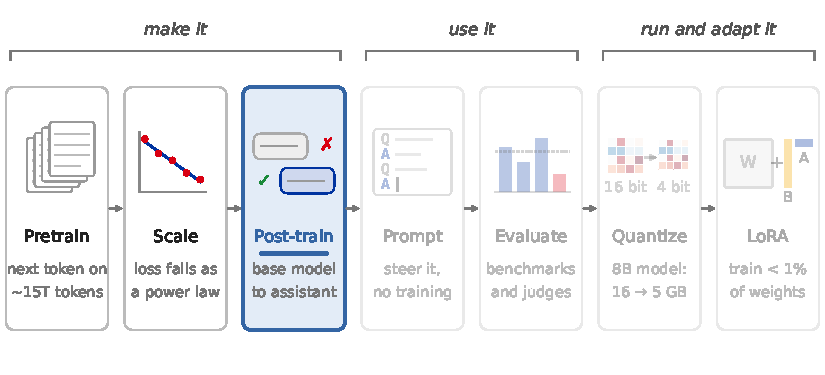
\includegraphics[width=\linewidth]{roadmap_post_training_life.pdf}\end{center}
  \vskip -2pt
  {\small Next (LLM-9): from a base model that continues documents to an assistant that answers.}
\end{frame}

\begin{frame}{Sources \& further reading}
  \footnotesize
  \begin{itemize}
    \item Kaplan et al. (2020), ``Scaling Laws for Neural Language Models''.
    \item Hoffmann et al. (2022), ``Training Compute-Optimal Large Language Models'' (Chinchilla);
      Besiroglu et al. (2024), ``Chinchilla Scaling: A replication attempt''.
    \item Rajbhandari et al. (2020), ``ZeRO'' (the 16 bytes per parameter).
    \item Brown et al. (2020), GPT-3; Llama Team (2024), ``The Llama 3 Herd of Models''.
    \item Wei et al. (2022), ``Emergent Abilities of Large Language Models''; Schaeffer, Miranda \&
      Koyejo (2023), ``Are Emergent Abilities of Large Language Models a Mirage?''.
    \item Power et al. (2022), ``Grokking''; Nanda et al. (2023), ``Progress measures for
      grokking''; Welch Labs (2025), ``Grokking'' (video).
  \end{itemize}
  \vskip 2pt
  \src{Figures: \texttt{py\_src/scaling\_figs.py} (published fits and sizes; the mirage curve is a
  toy). The grokking still: Welch Labs.}
\end{frame}

\end{document}

% ============================================================================
% Provenance:
%   Deck: LLM-8 Scaling laws and emergence (14_llms), session 8. Built 2026-10-06 from
%   LLM8_scaling_OUTLINE.md, which follows the critique in LLM_CHAPTER_PLAN.md (LLM-8) and the
%   recommended answers in INTERVIEW_QUEUE.md (instructor: "do all queue items"): kept separate
%   (DECISIONS #73), Chinchilla vs Gopher cold open, the mirage toy, one grokking frame.
%   Sources ported: dl4nlp 13 (Kaplan, Chinchilla vs Gopher, 6ND, 16 bytes) and 17 (Wei, Schaeffer,
%   grokking; the nature analogies, "three eras" and the AND-gate frame cut); llm_training 09.
%   Facts checked 2026-10-06 (outline table): Chinchilla abstract (67.5% vs 60.0%, "doubling");
%   the replication's parameter table; Power et al.'s step counts (local paper text).
%   Measured here: Hoffmann's published fit (eq. 10) puts the optimum at 50 tokens/parameter at
%   10^21 FLOPs and 93 at Chinchilla's budget; the 2024 refit at 22 and 18 (grid search in
%   scaling_figs.py, asserted). Every printed number is asserted there (6ND for both models,
%   2^-0.076, 2.5e19, 2.9B / 58B, 2.0 GB / 128 GB, tokens per parameter, p^5).
%   The grokking still is Welch Labs' frame f02 (misc/grokking/frames), copied to
%   fig/borrowed/welchlabs/grokking_curves.jpg; it shows Welch Labs' own run, described as such.
%   STUDENT REVIEW 2026-10-06 (one Sonnet agent, rendered PNGs only; ~82k tokens, 93 s). It re-did
%   every calculation (6ND x2, 2^-0.076, 2.5e19, 2.9B / 58B, sqrt 10, 16 bytes, 2.0 / 128 GB,
%   tokens per parameter, p^5) and found none wrong; it also confirmed the 0.66 per 10x against
%   the iso-FLOP dots. Applied: the floor's source and a bridge between Kaplan's 0.076 (model size
%   alone) and the fit's 0.66 (compute, above the floor); FLOPs and MMLU glossed at first use
%   ("within 20%", % correct, 25% by guessing); the fit's three terms in words and the quote's
%   attribution; the by-hand rule checked on Chinchilla itself (5.9e23 -> 70B, 1.4T, asserted);
%   the fit-check frame says what was fitted and what 22 / 18 are; sizes on the over-training
%   frame; the mirage's independence assumption, "% correct" axes, "those jumps"; the grokking
%   still described as a different setup (~60x) next to Power et al.'s ~1,000x, and the lesson
%   narrowed to "training loss cannot tell"; bf16, activations, two GPUs; the iso-FLOP caption off
%   the curves; "a preview" on the test-time frame.
% ============================================================================
